\documentclass[10pt,twocolumn,letterpaper]{article}

\usepackage{cvpr}
\usepackage{times}
\usepackage{epsfig}
\usepackage{graphicx}
\usepackage{amsmath}
\usepackage{amssymb}
\usepackage{caption}
\usepackage{subcaption}
\usepackage{booktabs}
\usepackage{makecell}
\usepackage{algorithm}
\usepackage[noend]{algpseudocode}

% Include other packages here, before hyperref.

% If you comment hyperref and then uncomment it, you should delete
% egpaper.aux before re-running latex.  (Or just hit 'q' on the first latex
% run, let it finish, and you should be clear).
\usepackage[pagebackref=true,breaklinks=true,letterpaper=true,colorlinks,linkcolor=blue,citecolor=blue,bookmarks=false]{hyperref}

\newcommand{\TODO}[1]{\textcolor{green}{#1}}
\newcommand{\CHANGED}[1]{\textcolor{red}{#1}}

%%%%%%%%% PAPER ID  - PLEASE UPDATE
\def\cvprPaperID{0125} % *** Enter the CVPR Paper ID here
\def\httilde{\mbox{\tt\raisebox{-.5ex}{\symbol{126}}}}

\begin{document}

%%%%%%%%% TITLE - PLEASE UPDATE
\title{Rebuttal for `Guided Proofreading of Automatic Segmentations for Connectomics'}  % **** Enter the paper title here

\maketitle
\thispagestyle{empty}

Thank you for your time and feedback.

\paragraph{R2: Venue} R2 writes ``While solid work, the paper is not a perfect fit for CVPR''. Biological and Cell Microscopy Image Analysis is included in the call for papers of CVPR 2018, and the field of connectomics has previously given rise to interesting papers at CVPR (Kumar~\etal 2010, Kaynig~\etal 2010, Jain~\etal 2010, Funke~\etal 2012, Pape~\etal 2017). %We believe our method will also be interesting to researchers working on tasks beyond connectomics, as segmentation proofreading for labeled dataset collection and correction is widely applicable in computer vision.

\paragraph{R2: Algorithmic Contribution/Innovation} R2 finds that the algorithmic contribution of our work is limited and less innovative. While we use a traditional CNN architecture, the GP framework can work with many classifiers and we believe is a promising direction to proofread segmentations more efficiently (lines 145-151).

\paragraph{R2: Superhuman Accuracy on the SNEMI3D Challenge} R2 misses the comparison to Lee~\etal~\cite{superhuman_performance} and asks whether proofreading is still competitive. Lee~\etal indeed report fantastic performance with their segmentation method but they also state the need for proofreading as future directions~\cite[sec. 8.2]{superhuman_performance}. We will integrate this discussion into the manuscript.

\paragraph{R2: Variation of Information Metric} R2 wishes to see the results reported using the adapted Rand Error metric (aRE). We originally chose variation of information (VI) to overcome some previously reported limitations of aRE \cite[p. 5]{NunezIglesias2013Machine} but will include aRE numbers as part of the supplemental material as reported in Table~\ref{tab:randerror}.

%\begin{figure}[h]
%\begin{center}
%  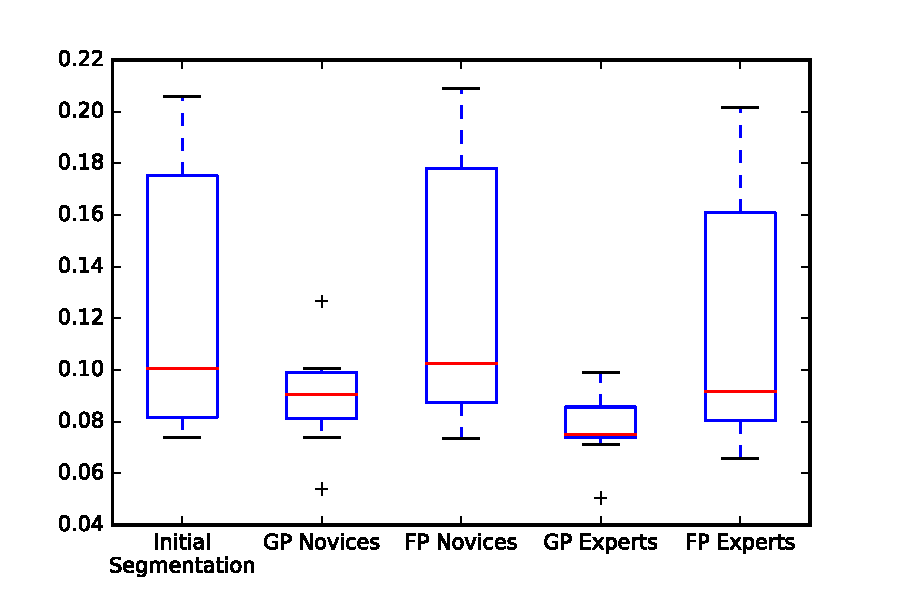
\includegraphics[width=\linewidth]{gfx/are_plot.pdf}
%\end{center}
%\vspace{-4mm}
%   \caption{Adapted Rand Error distributions of novices and experts using guided proofreading (GP) and focused proofreading (FP) as part of the forced choice user experiment across slices of the AC4 subvolume.}
%\label{fig:randerror}
%\end{figure}
\begin{table}[h]
\caption{The results of the Forced Choice User Experiment reported using the adapted Rand Error (aRE) metric, the lower the better. Novices and experts using GP perform better than using FP.}
\resizebox{\linewidth}{!}{
\begin{tabular}{lcccccccccc}
\toprule
% & \multicolumn{10}{c}{adapted Rand Error (aRE) per AC4 Subvolume slice} \\
% \midrule
Slice & 1 & 2 & 3 & 4 & 5 & 6 & 7 & 8 & 9 & 10 \\
\midrule
\emph{Init. Segm.} & 0.074 & 0.081 & 0.085 & 0.079 & 0.103 & 0.098 & 0.176 & 0.188 & 0.206 & 0.174 \\
\midrule
\emph{FP Novices} & 0.073 & 0.082 & 0.086 & 0.091 & 0.102 & 0.103 & 0.182 & 0.184 & 0.209 & 0.167 \\
\emph{GP Novices} & 0.054 & 0.074 & 0.083 & 0.081 & 0.100 & 0.086 & 0.127 & 0.095 & 0.100 & 0.096 \\
\midrule
\emph{FP Experts} & 0.066 & 0.080 & 0.078 & 0.087 & 0.083 & 0.096 & 0.163 & 0.174 & 0.202 & 0.155 \\
\emph{GP Experts} & 0.051 & 0.074 & 0.075 & 0.071 & 0.078 & 0.075 & 0.099 & 0.088 & 0.094 & 0.074 \\
\bottomrule
\end{tabular} 
}
\label{tab:randerror}
\end{table}








\paragraph{R2: Generalization of the AC4 Subvolume} R2 questions the generalization ability of the AC4 subvolume due to small dimensions. We agree that this dataset is small. However, it was introduced by Haehn~\etal 2014 for feasible interactive proofreading studies and is representative for the full AC4 dataset with respect to the distribution of object sizes.

\paragraph{R3: U-Net training data} R3 requests further information regarding the training data of the U-Net membrane probability classifier. Section 2 of the supplemental material includes this information (supplemental material lines 140-161, Table 3). We will modify the manuscript (lines 492-493) to include a direct reference.

\paragraph{R3: Generalization to other segmentation problems} R3 misses a  discussion regarding applicability of GP to general semantic segmentation problems. We believe our method will also be interesting to researchers working on tasks beyond connectomics, as segmentation proofreading for labeled dataset collection and correction is widely applicable in computer vision. We state mandatory re-training of GP for other datasets as a limitation in the supplemental material (lines 134-138) but will further elaborate on general segmentation problems in this section.

\paragraph{R3+R4: Network input channels} R3 is interested in seeing the performance contribution of the different input channels. R4 suggests that the membrane probabilities and the dilated border mask provide more discriminative information than the other two channels. We observe that all four input channels are important to reduce VI (Table~\ref{tab:input_channels}). Similar as identified by Bogovich~\etal, image data adds intracellular structures (e.g. vesicles) to the decision process and membrane probabilities include global knowledge of the staining protocol to highlight cell membranes. We then notice, that the label channel provides knowledge about neuron shapes while the border mask covers the gap of extra-cellular space.

\begin{table}[h]
\caption{We evaluate automatic selection on the AC4 subvolume ($p_t=0.95$) using the GP classifier with different input channels and report median VI reduction. The combination of all four channels performs best.}
\resizebox{\linewidth}{!}{
\begin{tabular}{lrrrr}
\toprule
\makecell{Input channels} & \makecell{VI reduction} \\
\midrule
\emph{Image + Prob.} &  -0.094\\
\emph{Image + Prob. + Border} & -0.045\\
\emph{Image + Prob. + Label} & 0.038\\
\emph{Image + Prob. + Label + Border} & 0.065\\
\bottomrule
\end{tabular} 
}
\label{tab:input_channels}
\end{table}

\paragraph{R4: Dilated mask of the border between two segments} R4 raises the question of whether the dilated mask of the border is a crucial input to our classifier. The dilated border improves classifier performance measured as VI reduction from $0.038$ to $0.065$ (Table~\ref{tab:input_channels}). We qualitatively describe the intention behind the border mask in lines 315-323 but will add the experiment above to the supplemental material and to the open source repository.

\paragraph{R4: 2D Slices only} R4 observes that GP works in 2D. We report this limitation and a proposed solution in the supplemental material lines 129-133 and will add a direct reference to the manuscript. However, 2D processing enables segmentation and proofreading in parallel to 2D image acquisition prior to any expensive 3D alignment.

\paragraph{R4: Merge error detection performance} R4 expresses concerns regarding the performance contribution of merge error correction. Typical connectomics segmentations begin with an over-segmentation (lines 498-499), in which we attempt to find all possible cell boundary edges. At this stage, some edges are missed due to low contrast - these missing edges cause merge errors. To correct this, we need to imagine where any number of edges might be among empty space, and this is simply a harder visual task than assessing whether an identified edge is correct. This is true even for a human: on the AC4 dataset, our experts only agree with the selection oracle in two thirds of merge error cases.


{\small
\bibliographystyle{ieee}
\bibliography{../../connectomics}
}

\end{document}
